\documentclass[12pt]{article}
\usepackage[a4paper, total={6in, 10in}]{geometry}


\usepackage{graphicx}
\graphicspath{{/home/map479/mxochicale/github/3minutethesis/3minutesthesisrepository/rehearsals/images/}}


\usepackage[counterclockwise]{rotating} %sidewaysfigure

\author{Miguel P Xochicale}
\title{ Are Robots the Future of Elder Care?  } 
\date{\today}

\begin{document}
\maketitle

If you are lucky enough, you will live an average of 80 years.
But, have you ever wondered how would it be turning 60, 70, 80 or maybe 90 years old?
Now, think about as we are ageing, we will be gradually losing all our
charming human senses such as sight, hearing, taste, smell, and touch.
In short, both our motor and cognitive skills will be diminished as we age.

Now think about the people who will be with you until the last day.
Will they be with you at all 
and most importantly will they take care of you?

And how about the global view of people who are ageing.
According to the 2017 revision of the world population prospects[1], 
people aged 60 years or over
is expected to be more than double by 2050 and to be more than triple by 2100[2].

Well, you don`t have to worry too much in the coming years, 
because here it is where caregiver robots come up.
In the last decade, experimental robots, mainly Japannese ones, help lift people into and out of their chairs and beds,
follow recipies for cooking, fold towels or even dispense pills[3].
Recently, in the last five years robots like
Paro, a small humanoid robot, can play games and dance with the eldery
and therefore keep their minds activite.
Another example is Pepper, a personal humanoid robot, that has the power 
to read and respond to human emotions[0]
and the list goes on and on.

Generally speaking, caregiver robots can meet our physical and emotional needs as we age,
by offering reminders about appointments, medications 
and encourages social activity, healthy eating and exercise[4].

That is the future that I am working on.
A future where humanoids robots with the use of sensors can understand human movement and emotions.
Particularly, in my PhD I have implemented and developed algorithms to measure 
variability of movement and emotions 
for which humanoid robots can enhance and monitor physical activities of the elderly[5].

Perhaps my parents, back in Mexico, are not going to be benefit 
from this technological advances 
but I do believe that future generations of people will be assisted by caregiver robots
and therefore making the elderly more independent, happier and healthier!

372 words. 



\newpage

\begin{sidewaysfigure}
\centering
\includegraphics{figure02}
\caption{3 minutes thesis figure}
\end{sidewaysfigure}



\end{document}
